%%%%%%%%%%%%%%%%%%%%%%%%%%%%%%%%%%%%%%%%%
% 11/26 4faW13M 
% Phy 499 report

\documentclass[letterpaper]{article}
\usepackage[paperwidth=8.5in, paperheight=11in]{geometry}
\linespread{1.5}
\normalsize

\usepackage[utf8]{inputenc}

\usepackage{indentfirst}
\usepackage[utf8]{inputenc}
\usepackage{geometry}

\usepackage{amsmath,amsfonts,amsthm} % Math packages
\newcommand{\thickhat}[1]{\mathbf{\hat{\text{$#1$}}}}
\newcommand{\thickbar}[1]{\mathbf{\bar{\text{$#1$}}}}
\newcommand{\thicktilde}[1]{\mathbf{\tilde{\text{$#1$}}}}

\usepackage[english]{babel}
\usepackage[autostyle]{csquotes}

%\usepackage{spverbatim}

\usepackage{listings}
\usepackage{lstautogobble}

\lstset{basicstyle=\ttfamily,
	mathescape=true,
	escapeinside=||,
	autogobble,
	xleftmargin=0.7in,
	xrightmargin=.25in}

\usepackage{graphicx}

\usepackage[export]{adjustbox}

\usepackage{amsfonts} % if you want blackboard bold symbols e.g. for real numbers

\usepackage{amsmath}
\usepackage{physics}

\usepackage{chngcntr}
\usepackage{wrapfig}
\usepackage{caption}
\usepackage{subcaption}

\usepackage{verbatim} % 4faW13

%\usepackage{subfig}




\numberwithin{equation}{section} % Number equations within sections (i.e. 1.1, 1.2, 2.1, 2.2 instead of 1, 2, 3, 4)
\numberwithin{figure}{section} % Number figures within sections (i.e. 1.1, 1.2, 2.1, 2.2 instead of 1, 2, 3, 4)
\numberwithin{table}{section} % Number tables within sections (i.e. 1.1, 1.2, 2.1, 2.2 instead of 1, 2, 3, 4)

\title{	
	\normalfont \normalsize 
	\huge The Spatial Correlations of the Noise
	\\ % The assignment title
}

\author{Ruojun Wang} % Your name

\date{\normalsize\today} % Today's date or a custom date

\begin{document}

\maketitle % Print the title

\section{Background}
Quantum noise refers to the uncertainty of a physical quantity that is due to its quantum origin. In terms of the measurement of noise correlations, quantum noises are due to decoherent states in an entangled system. Hence, errors could be caused in a result given by quantum computer due to noise. The existence of noise correlations could help correct errors.  

\section{Method}

\paragraph{Measurements.}
\enquote{Meassurement of SNC} suggests an experiment to measure the local noise spectra $S_{ij}$ with two measures ${T_2}^{(1)}$ and ${T_2}^{(2)}$. With ${T_2}^{(+)}$ and ${T_2}^{(-)}$ are characteristic time scale for the Ramsey experiments in the $\left\{\ket{00}, \ket{11}\right\}$ basis and those in the $\left\{\ket{01}, \ket{10}\right\}$ basis. The local noise spectra could then be calculated by $$\frac{1}{{T_2}^{\pm}}=\frac{1}{{T_2}^{(1)}}+\frac{1}{{T_2}^{(2)}}\pm \frac{8}{\hbar^2} \lim_{\omega\to 0} S_{12}(\omega)$$. \cite{Premakumar} The Ramsey experiments can be constructed with gate sequences on IBM Q website. By analysis of the data obtained from the Ramsey experiments, the four quantities ${T_2}^{(1)}$, ${T_2}^{(2)}$, ${T_2}^{(+)}$ and ${T_2}^{(-)}$ can be estimated. 

\begin{figure}
	\centering
	
	\begin{subfigure}[b]{0.8\textwidth}
		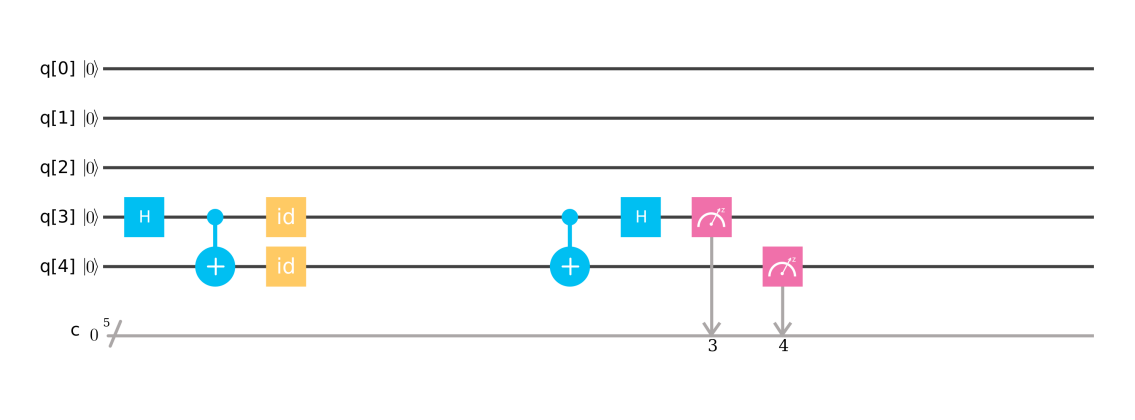
\includegraphics[width=\textwidth]{C00}
		\caption{00+11}
		\label{C00}
	\end{subfigure}
	
	\begin{subfigure}[b]{0.8\textwidth}
		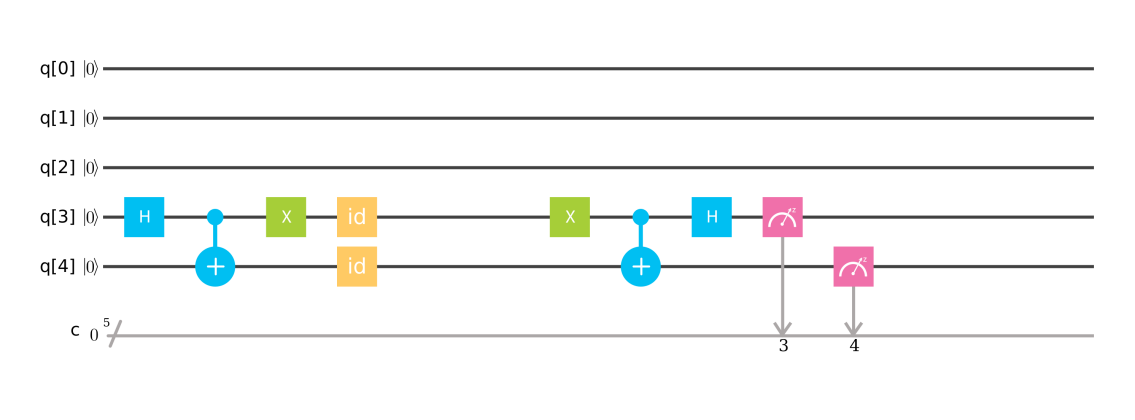
\includegraphics[width=\textwidth]{C01}
		\caption{01+10}
		\label{C01}
	\end{subfigure}
	
	\begin{subfigure}[b]{0.8\textwidth}
		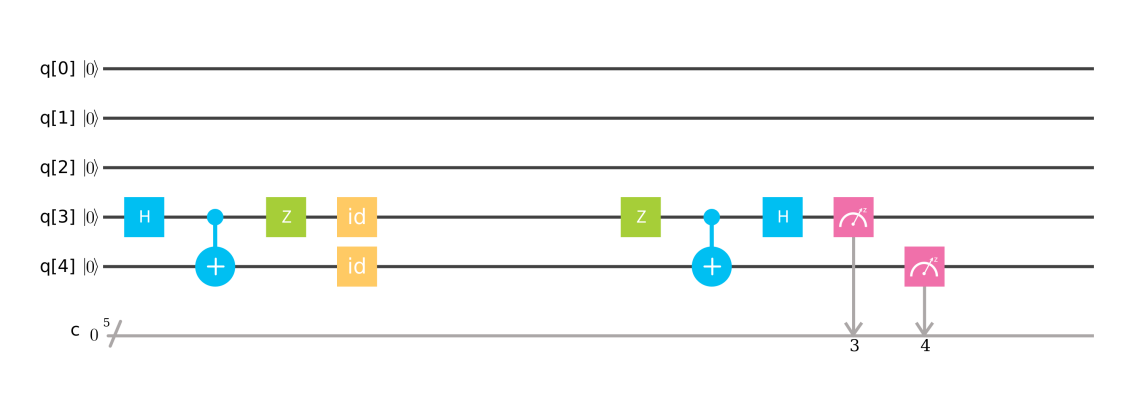
\includegraphics[width=\textwidth]{C10}
		\caption{00-11}
		\label{C10}
	\end{subfigure}
	
	\begin{subfigure}[b]{0.8\textwidth}
		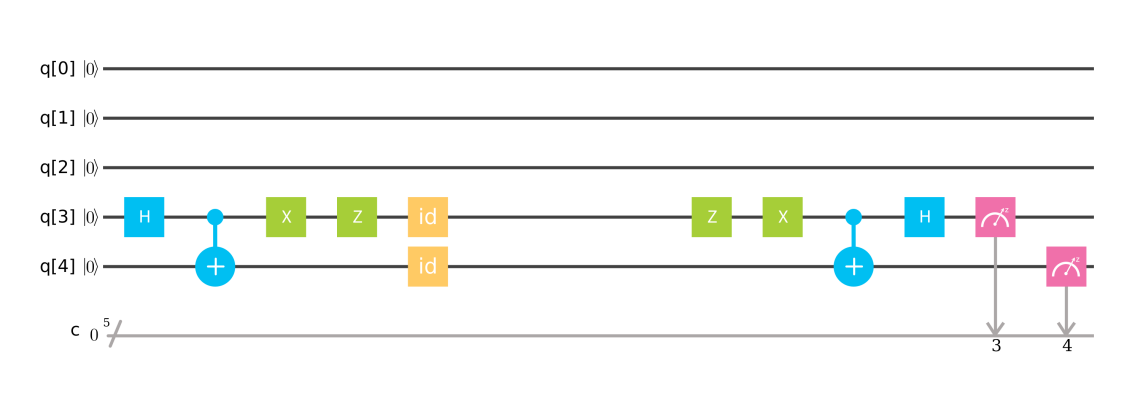
\includegraphics[width=\textwidth]{C11}
		\caption{01-10}
		\label{C11}
	\end{subfigure}
	
	\caption{Four bell states prepared by device on IBM Q}
	\label{4BS}
\end{figure}

\paragraph{Gate Sequence.}
Four gate sequences are shown in figure 2.1 to prepare four bell states. The \enquote{id} represents for the identity gate and functions as one unit time (the exact time is unknown for now). The number of identity gates controls the waiting time that a bell state would last before the state rotates back to the original direction in the Bloch sphere under the influence of later gate. To study how the distribution of four outcomes (00, 01, 10, 11), $n$ identity gates need to be inserted in the sequence. With the restriction of the number of gates, $n\leq74$ for 00+11 state and $n\leq71$ for 01+10 state. 



\section{Results}

For 00+11 state, I tableted the results of distributions for four outcomes and the calibration data (T1, T2). I fit the data with 2 functions: $C \exp(- \frac{t}{{T_2}^{(-)}})$ and $C \exp(- (\frac{t}{{T_2}^{(-)}})^2)$, where $C$ is a constant. However, the error between the data and the fitting curve is large so I added constants to the fitting function to minimize the error. 

I tableted 5 more groups of results for 00+11 state (8 groups in total) (figure 3.1, 3.2). I fit these with new functions with extra constants: $C \exp(- \frac{t}{{T_2}^{(-)}})+D$ and $C \exp(- (\frac{t}{{T_2}^{(-)}})^2+D)$ and $k t + b$, where $C$, $D$, $k$ and $b$ are constants. I also tableted two groups of outcomes for 01+10 state (figure 3.3). I fit these with the above three functions, where ${T_2}^{(-)}$ is replaced by ${T_2}^{(+)}$. 

\begin{figure}[h]
	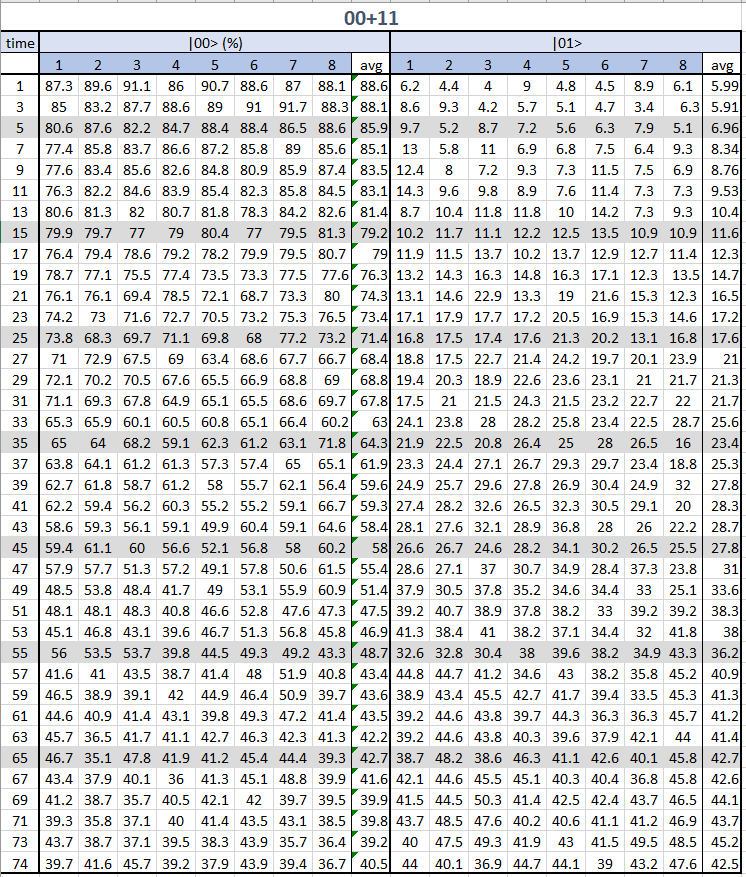
\includegraphics[width=\textwidth]{t00n11}
	\caption{A table for 00+11 bell state. The column "time" gives the number of identity gates, each of which functions as one unit time. $\ket{00}, \ket{01}$ are four outcomes given by this gate sequence. The second row marks the number of times that one experiment is run and the average of the outcomes given by the total 8 runs.}
	\label{t00n11}
\end{figure}

\begin{figure}[h]
	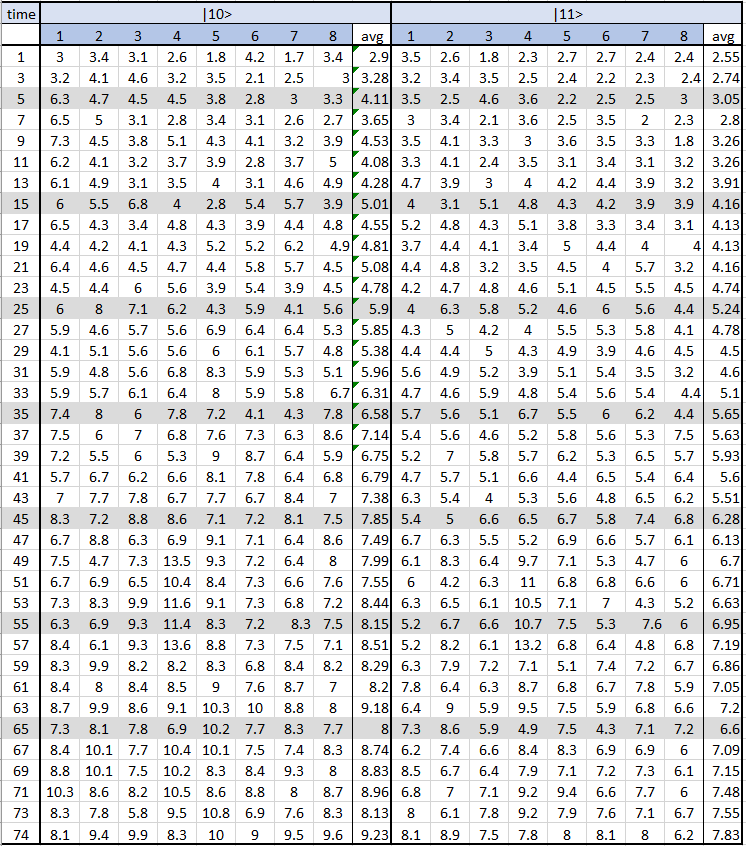
\includegraphics[width=\textwidth]{t00n11b}
	\caption{A table for 00+11 bell state which gives $\ket{10}, \ket{11}$ outcomes.}
	\label{t00n11 b}
\end{figure}

\begin{figure}[h]
	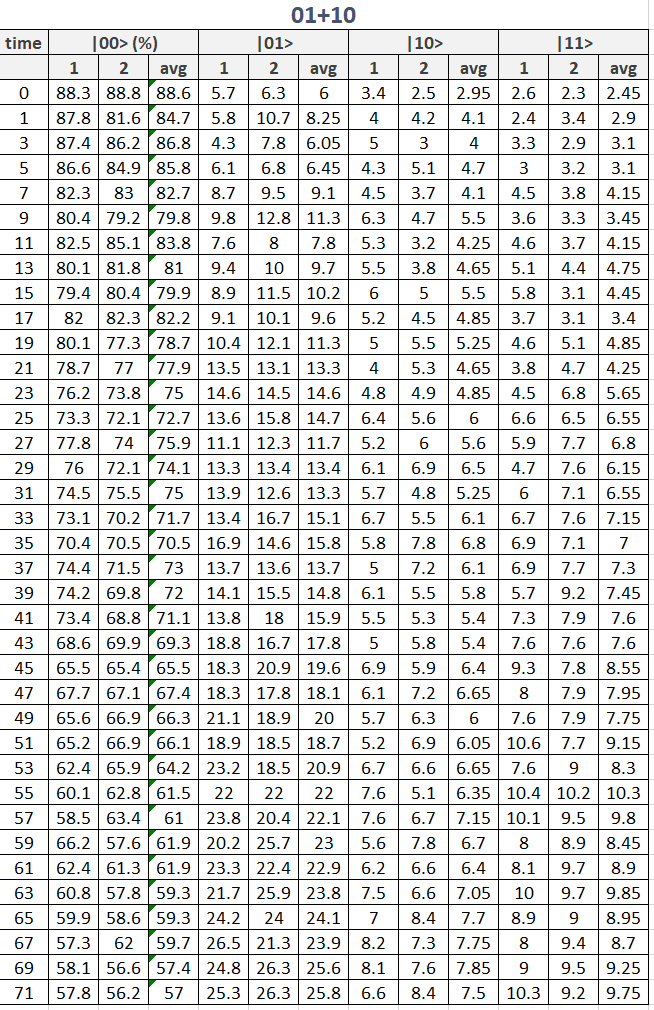
\includegraphics[width=120mm,scale=1.0]{t01n10}
	\caption{A table for 01+10 bell state which gives $\ket{00}, \ket{01}, \ket{10}, \ket{11}$ outcomes for total 2 runs.}
	\label{t01n10}
\end{figure}


\begin{comment}
\begin{figure}[t]
	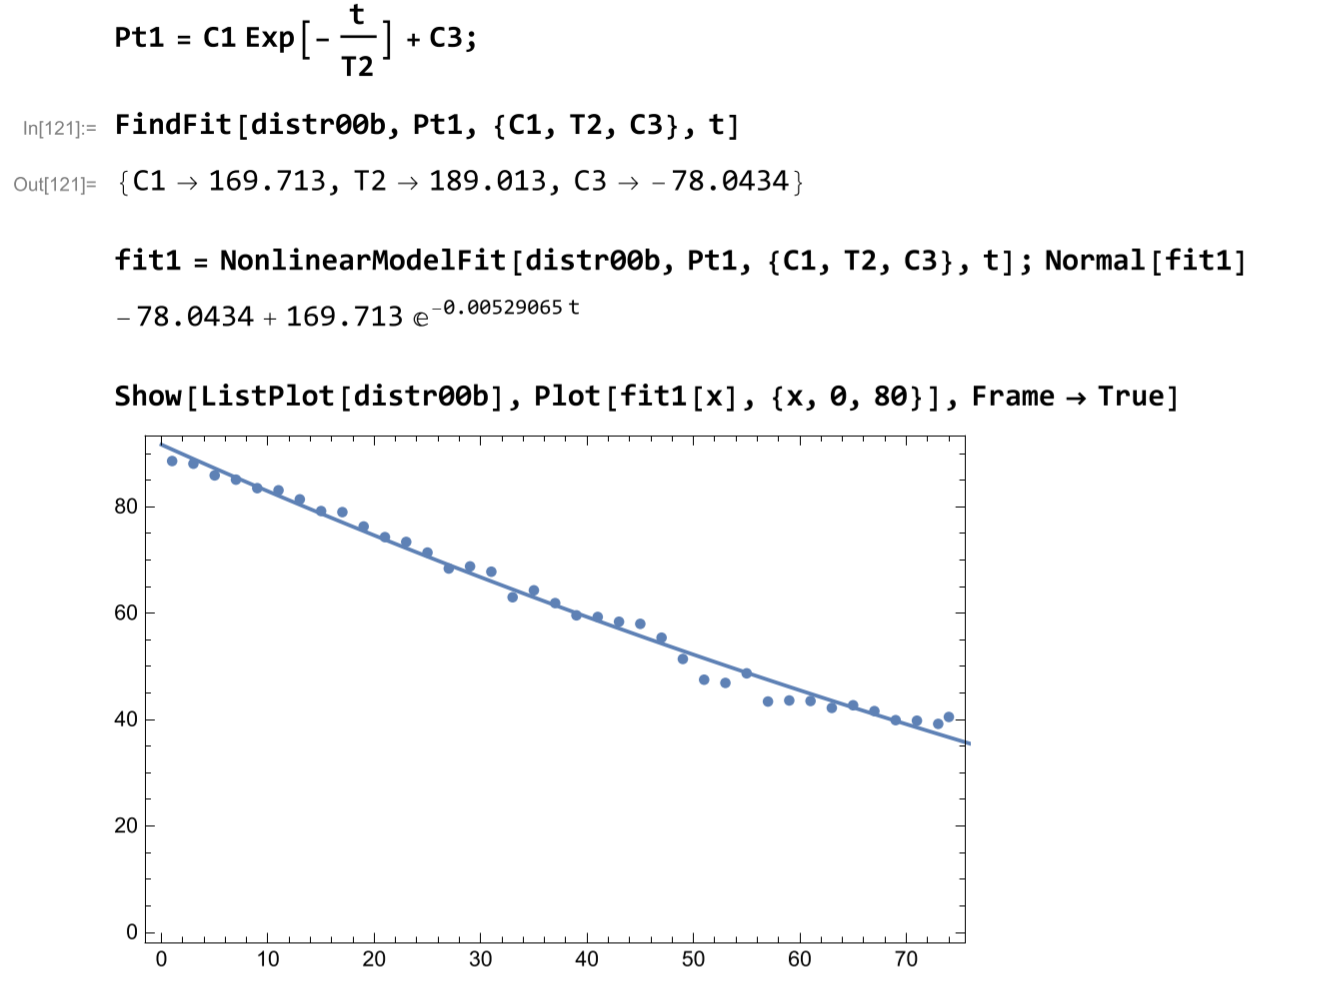
\includegraphics[width=120mm,scale=1.0]{00n11fitExp}
	\caption{}
	\label{00n11fitExp}
\end{figure}

\begin{figure}[t]
	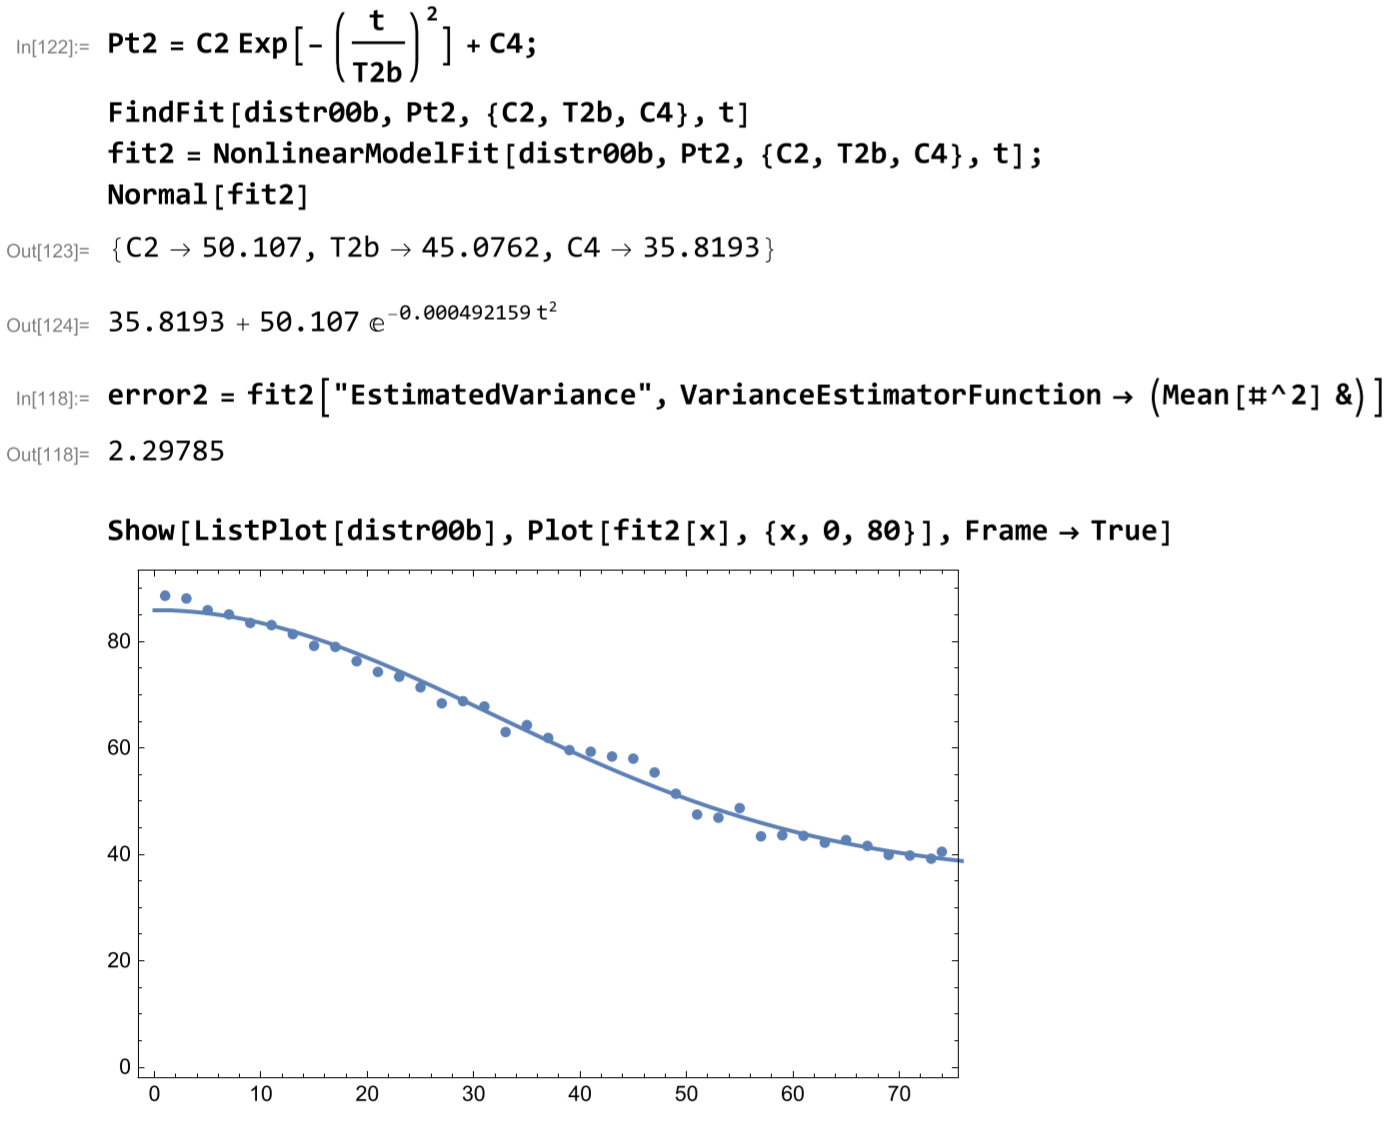
\includegraphics[width=\textwidth]{00n11fitExpSq}
	\caption{}
	\label{00n11fitExpSq}
\end{figure}

\begin{figure}[t]
	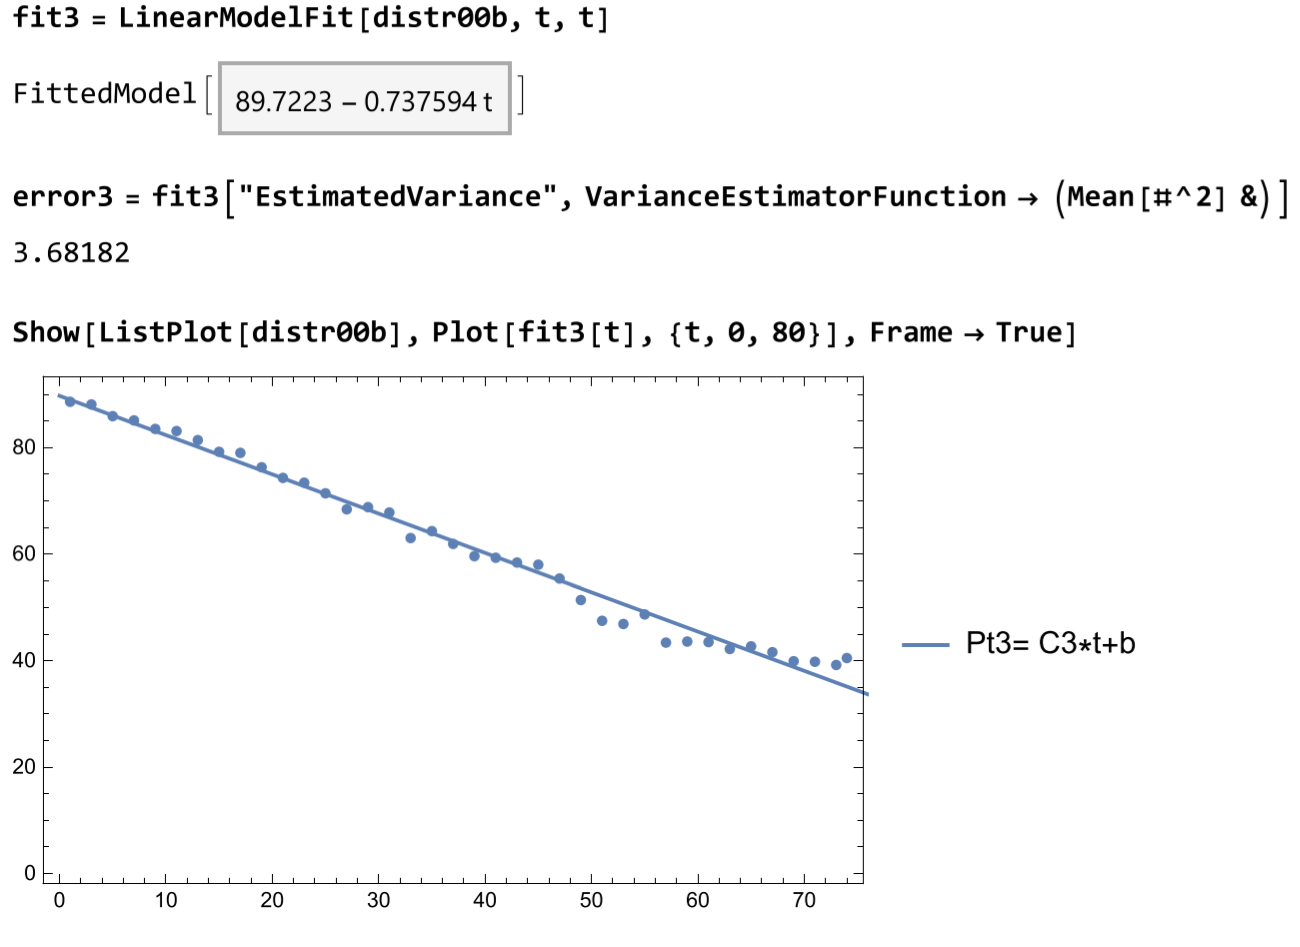
\includegraphics[width=\textwidth]{00n11fitLinear}
	\caption{}
	\label{00n11fitLinear}
\end{figure}



\begin{figure}[h]
	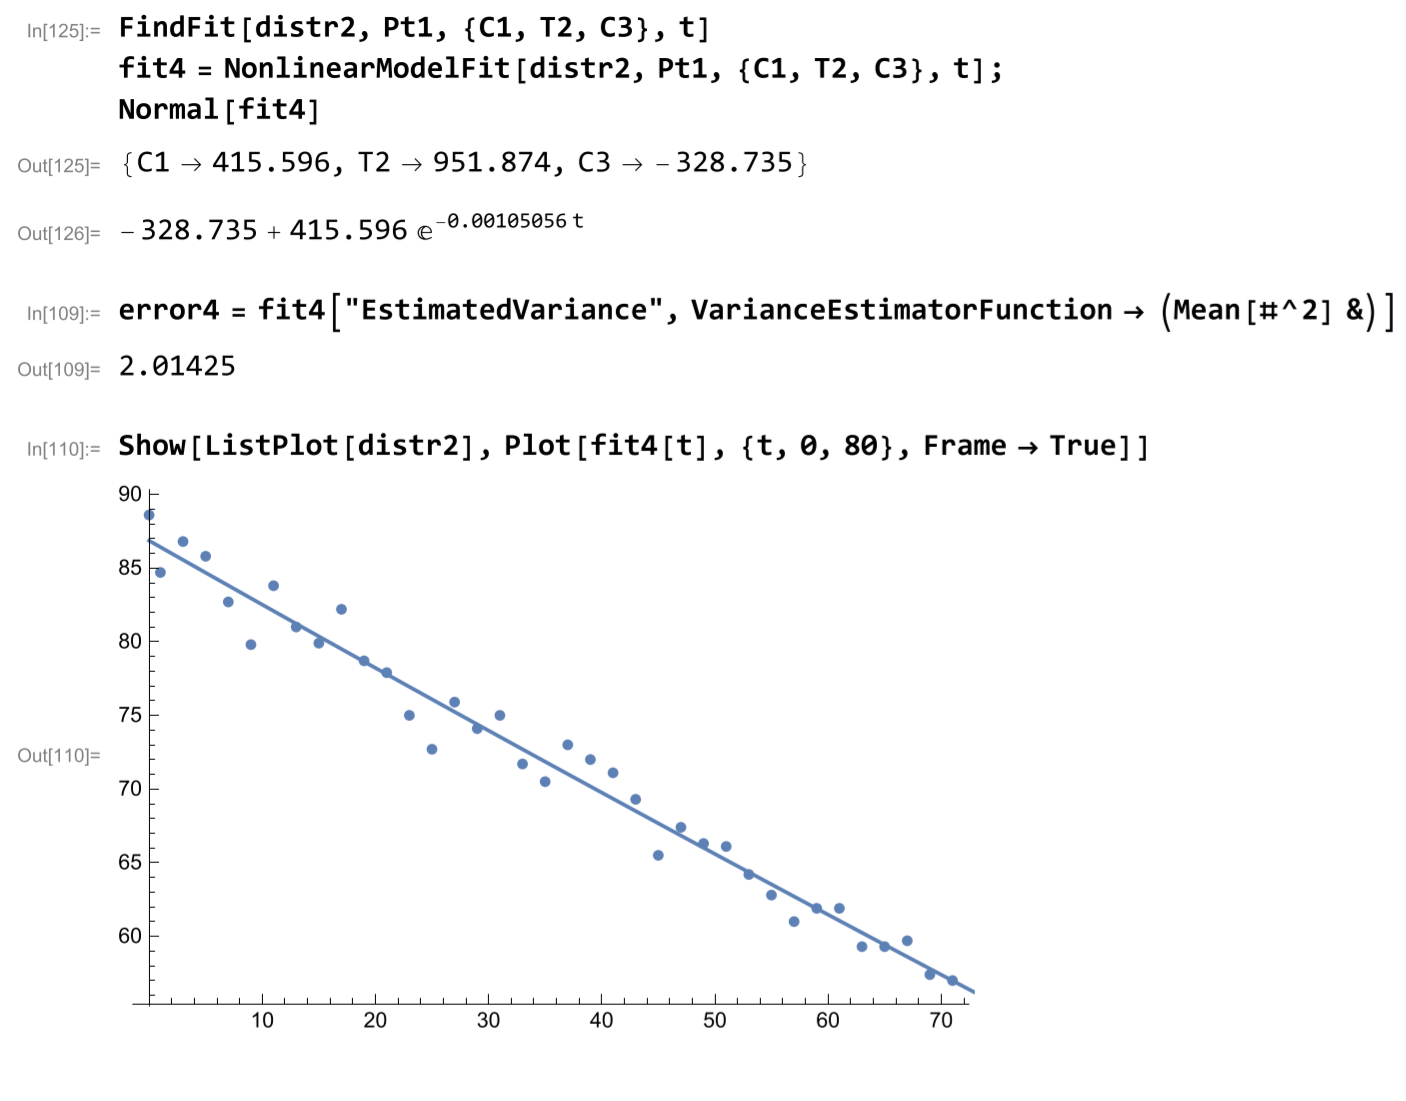
\includegraphics[width=\textwidth]{01n10fitExp}
	\caption{}
	\label{01n10fitExp}
\end{figure}

\begin{figure}[h]
	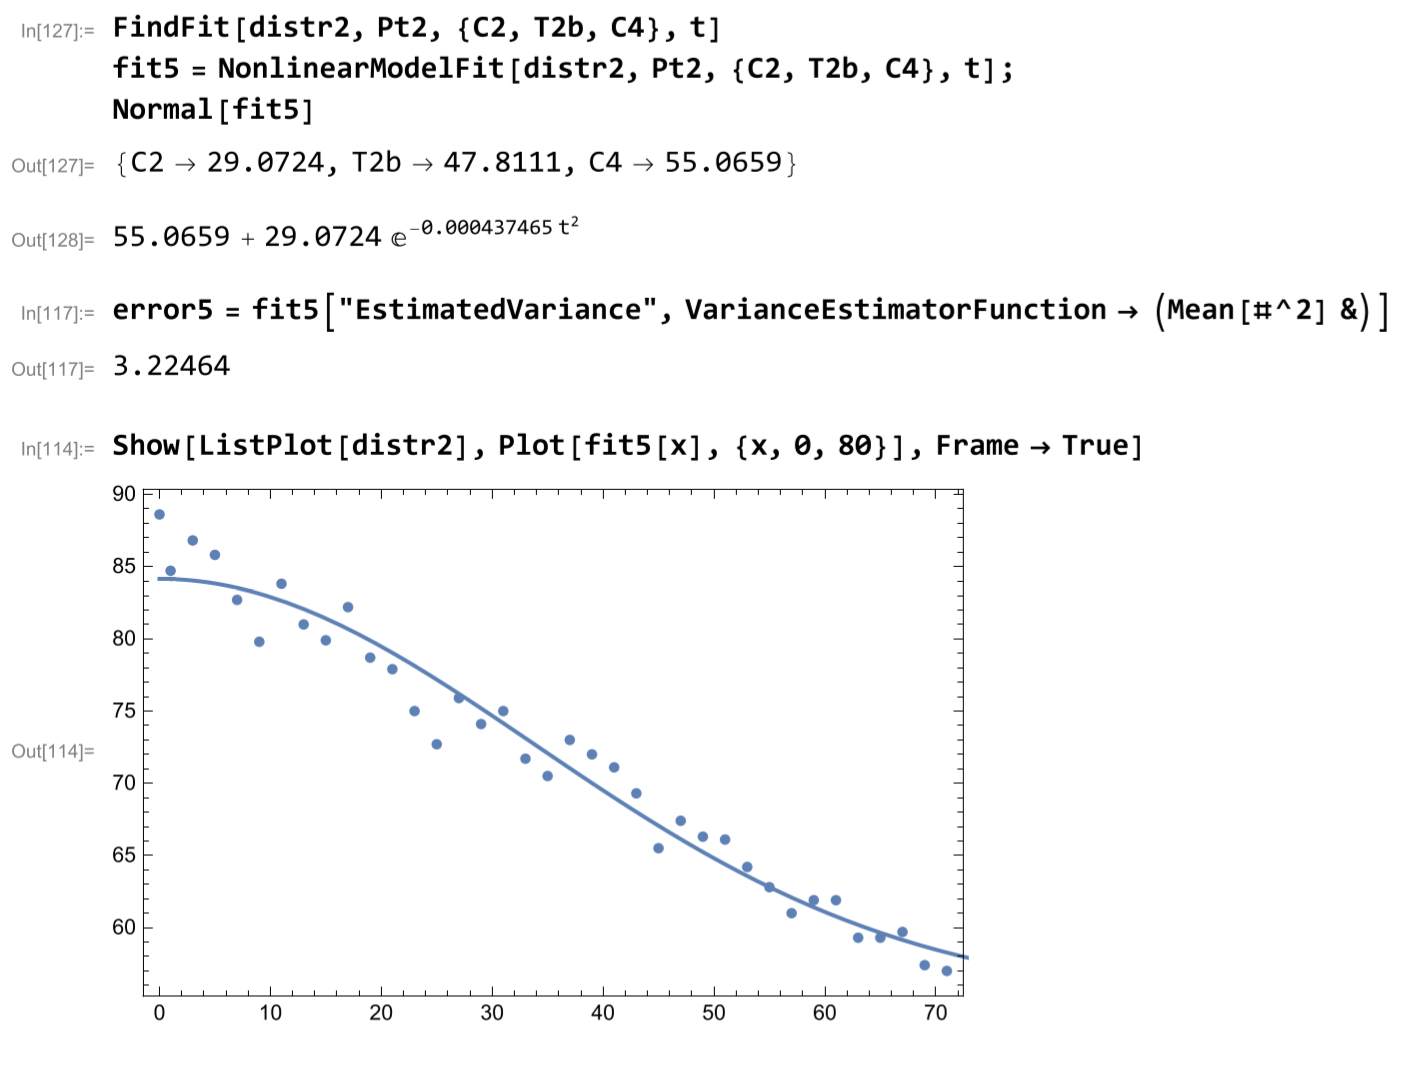
\includegraphics[width=\textwidth]{01n10fitExpSq}
	\caption{}
	\label{01n10fitExpSq}
\end{figure}

\begin{figure}[h]
	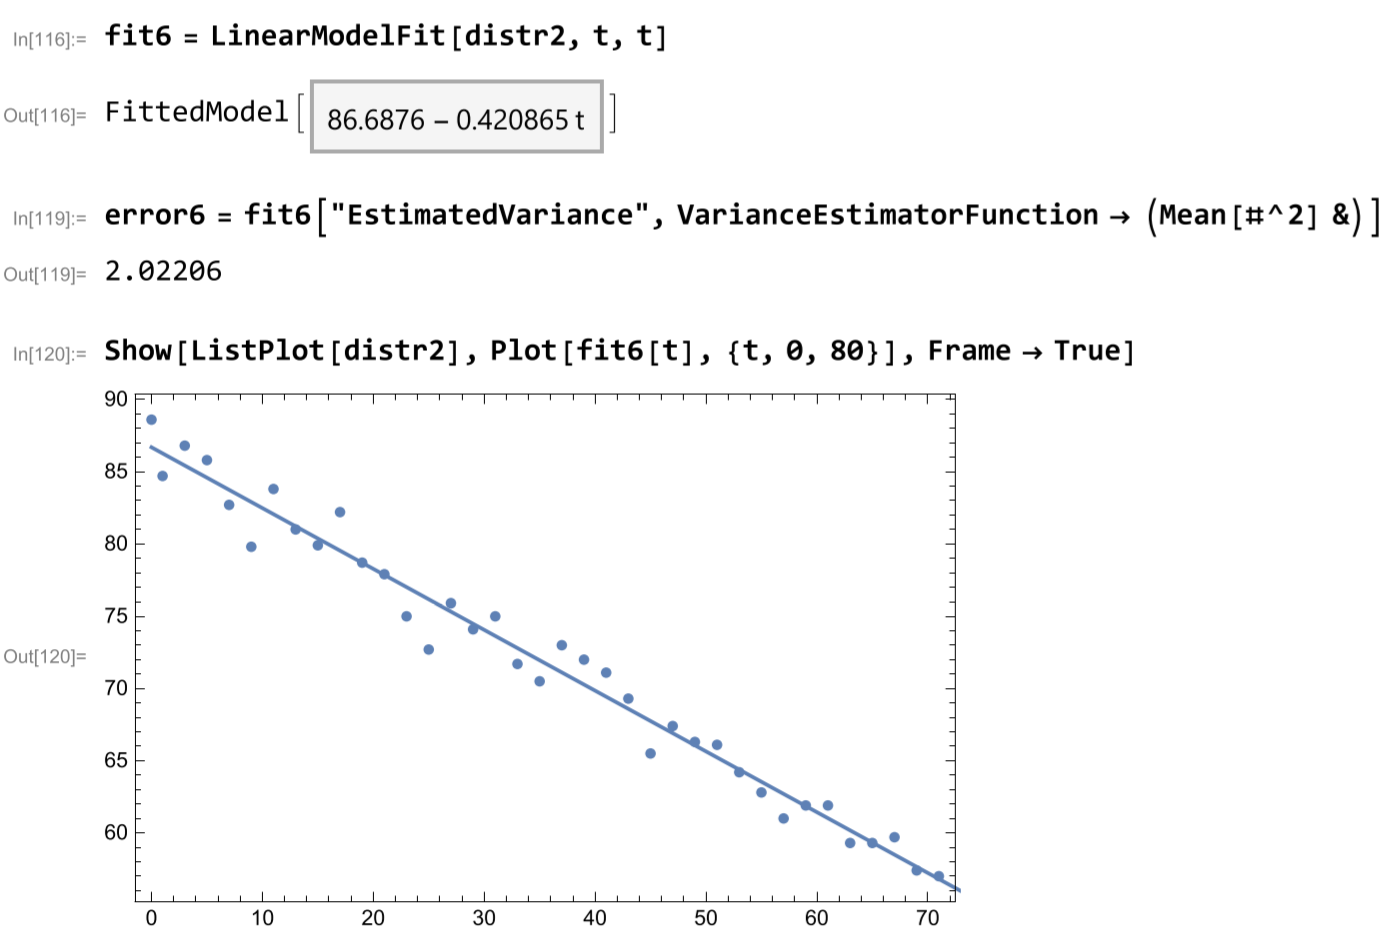
\includegraphics[width=\textwidth]{01n10fitLinear}
	\caption{}
	\label{01n10fitLinear}
\end{figure}
\end{comment}



\section{Conclusions}
Given the above analysis of data from Ramsey experiments, the variance of each fitting function is also computed. For 00+11 bell state, the variance of $C \exp(- \frac{t}{{T_2}^{(-)}}+D)$ is 2.92664, the one of $C \exp(- (\frac{t}{{T_2}^{(-)}})^2+D)$ is 2.29785 and the one of linear fitting is 3.68182. Hence, we obtain ${T_2}^{(-)} \approx 45.0762$ from the fitting of $C \exp(- (\frac{t}{{T_2}^{(-)}})^2+D)$. For 01+10 bell state, the variance of $C \exp(- \frac{t}{{T_2}^{(-)}}+D)$ is 2.01425, the one of $C \exp(- (\frac{t}{{T_2}^{(-)}})^2+D)$ is 3.22464 and the one of linear fitting is 2.02206. ${T_2}^{(+)} \approx 951.874$ is obtained from the first fitting. 


\begin{comment}
$$\frac{1}{{T_2}^{\pm}}=\frac{1}{{T_2}^{(1)}}+\frac{1}{{T_2}^{(2)}}\pm \frac{8}{\hbar^2} \lim_{\omega\to\infty} S_{12}(\omega)$$


\section{An IDLA Simulation and the Boundary}

\subsection{An IDLA Simulation with N Particles}



\subsubsection{Particles move in 8 directions}


	



\begin{comment}
\paragraph{Build entire boundary.}


\begin{align} 
(\Delta f)_{i,j} = 4f_{i,j}-f_{i+1,j}- f_{i-1,j}-f_{i,j+1}-f_{i,j-1},
\end{align}


\noindent
where $i$ and $j$ here represent the horizontal and vertical coordinate of the center of one grid. Similarly to the second algorithm, the grids which are occupied are marked as "1," and those which are not occupied are denoted as "0." Hence, if $(\Delta f)_{i,j}>0$, the grid with coordinate $(i,j)$ is considered on the boundary. 
\end{comment}


\begin{comment}

\end{comment}

\begin{comment}
\begin{figure}[b]{1.0\textwidth}
	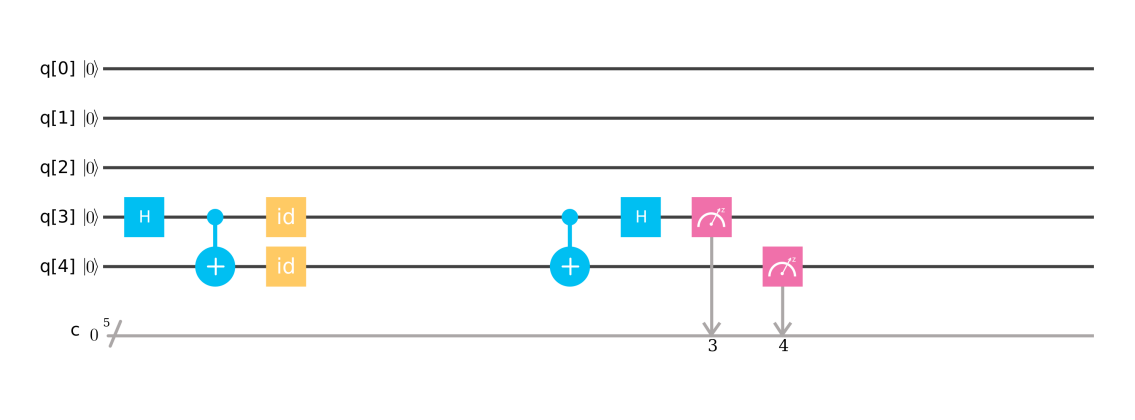
\includegraphics[width=\textwidth]{C 00.png}
	\caption{00+11}
	\label{C 00}
\end{figure}

\begin{figure}[b]{1.0\textwidth}
	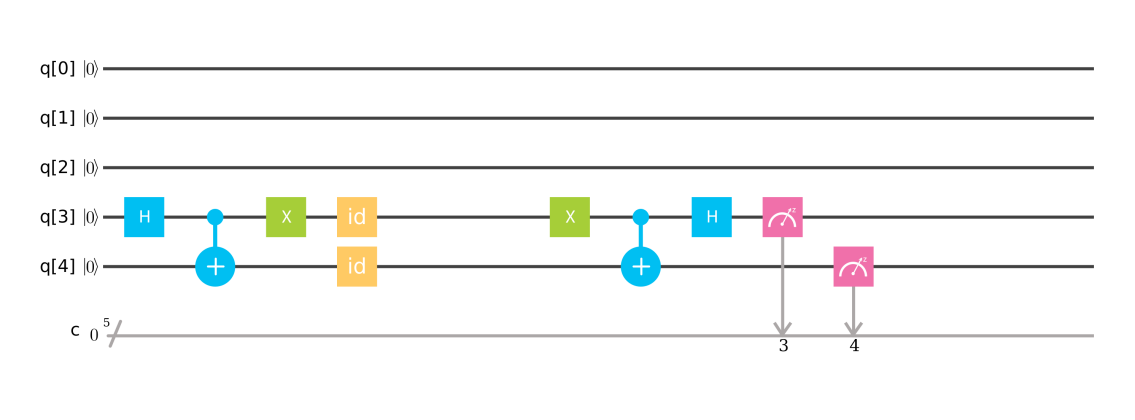
\includegraphics[width=\textwidth]{C 01.png}
	\caption{01+10}
	\label{C 01}
\end{figure}

\begin{figure}[b]{1.0\textwidth}
	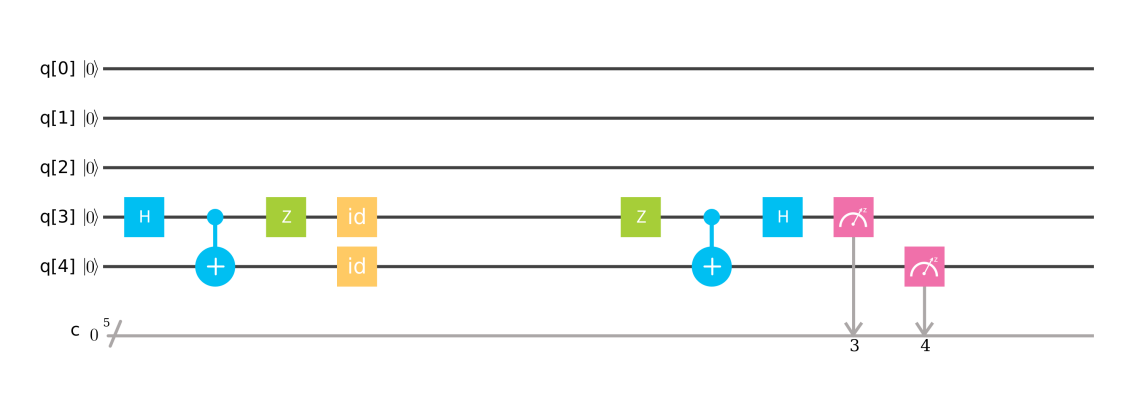
\includegraphics[width=\textwidth]{C 10.png}
	\caption{00-11}
	\label{C 10}
\end{figure}

\begin{figure}[b]{1.0\textwidth}
	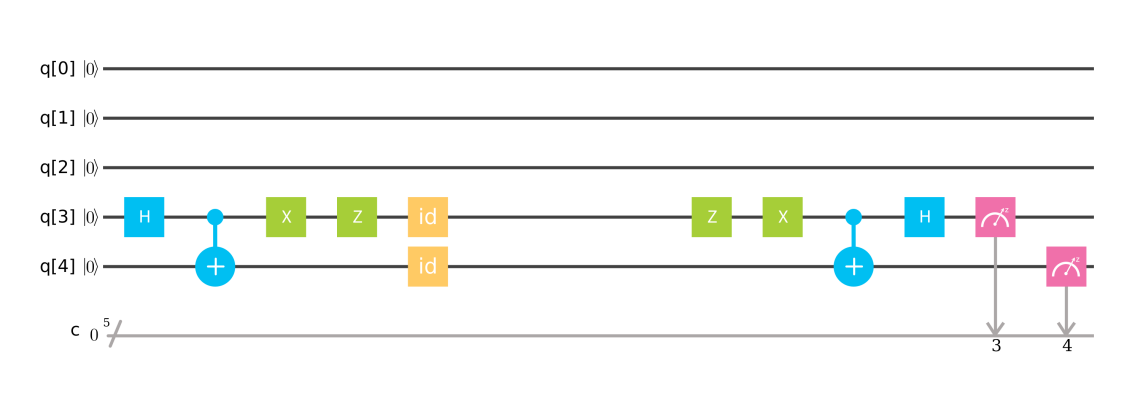
\includegraphics[width=\textwidth]{C 11.png}
	\caption{01-10}
	\label{C 11}
\end{figure}
\end{comment}



\begin{thebibliography}{9}
	\bibitem{Premakumar} 
	Vickram N. Premakumar, H. Ekmel Ercan, Joydip Ghosh, Mark Friesen, M.A. Eriksson, S.N. Coppersmith, and Robert Joynt. 
	Measurement of SNC. 
	(...), 2018.
\end{thebibliography}







\end{document}